In this section, we correctly place corners. This completely solves the top layer as shown in \figref{toplayer}.
\begin{figure}[h]
	\centering
	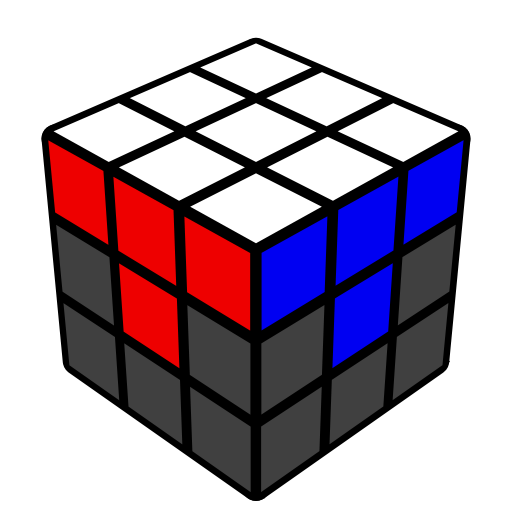
\includegraphics[width=0.3\textwidth]{toplayer.png}
	\caption{Solved top layer}\label{fig:toplayer}
\end{figure}
\begin{enumerate}
	\item Find an unsolved corner piece and bring it to the bottom layer.
	\item Twist the bottom layer to bring it underneath where it is supposed to go. It will then be in one of the configurations shown in \figref{confs}.
\begin{figure}[h]
	\centering
	\begin{subfigure}[b]{0.3\textwidth}
		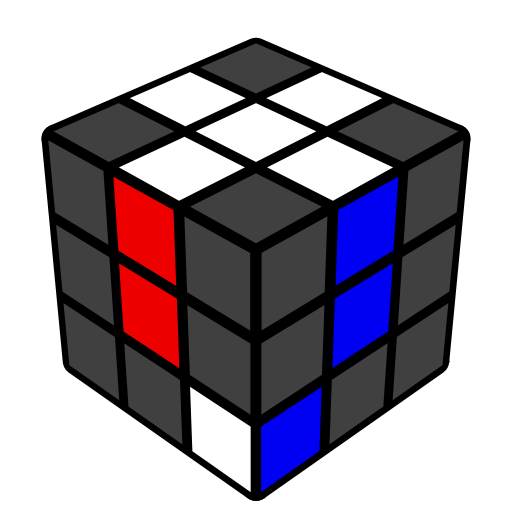
\includegraphics[width=\textwidth]{conf1.png}
	\end{subfigure}
	\begin{subfigure}[b]{0.3\textwidth}
		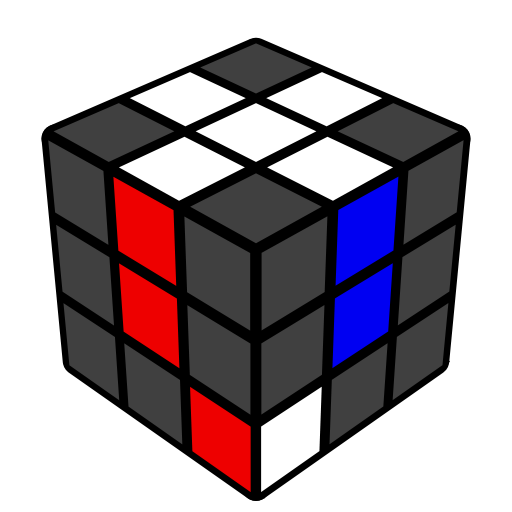
\includegraphics[width=\textwidth]{conf2.png}
	\end{subfigure}
	\begin{subfigure}[b]{0.3\textwidth}
		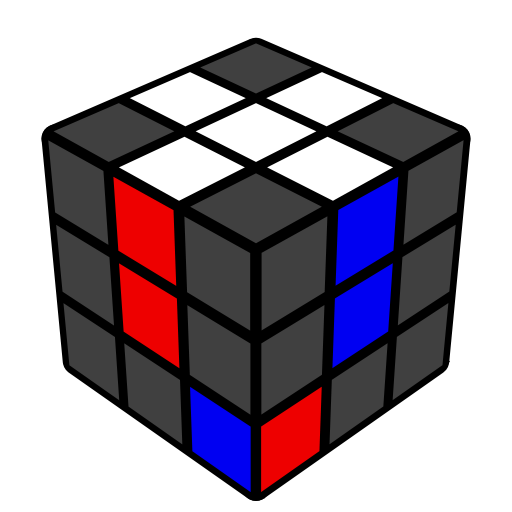
\includegraphics[width=\textwidth]{conf3.png}
	\end{subfigure}
	\caption{Possible configurations of the corner piece.}\label{fig:confs}
\end{figure}
	\item Hold the cube so that the corner appears at the bottom-right of the front face.
	\item Perform the algorithm \alg{R'D'RD} repeatedly until the corner is solved.
	\item Repeat from step 1 until all corners are solved.
\end{enumerate}